\chapter{Implemented Solution}
\section{Amazon Web Services}

\subsection{Architecture}
Since Amazon Elastic Beanstalk has been used as the core component to organize the system, it has been possibile to use an Infrastructure as a Service grade of customization, with an easier configuration and building phase as if the system were Platform as a Service instead.\\
As shown in the picture \ref{fig:architecture}, everything but the SES service is hosted in the eu-central-1 region in Frankfurt, which is divided into availability zones connected through low-latency links, in order to handle potential instance failures by replacing those failed with the standby ones, placed in a different availability zone.\\

\begin{figure}[h]
    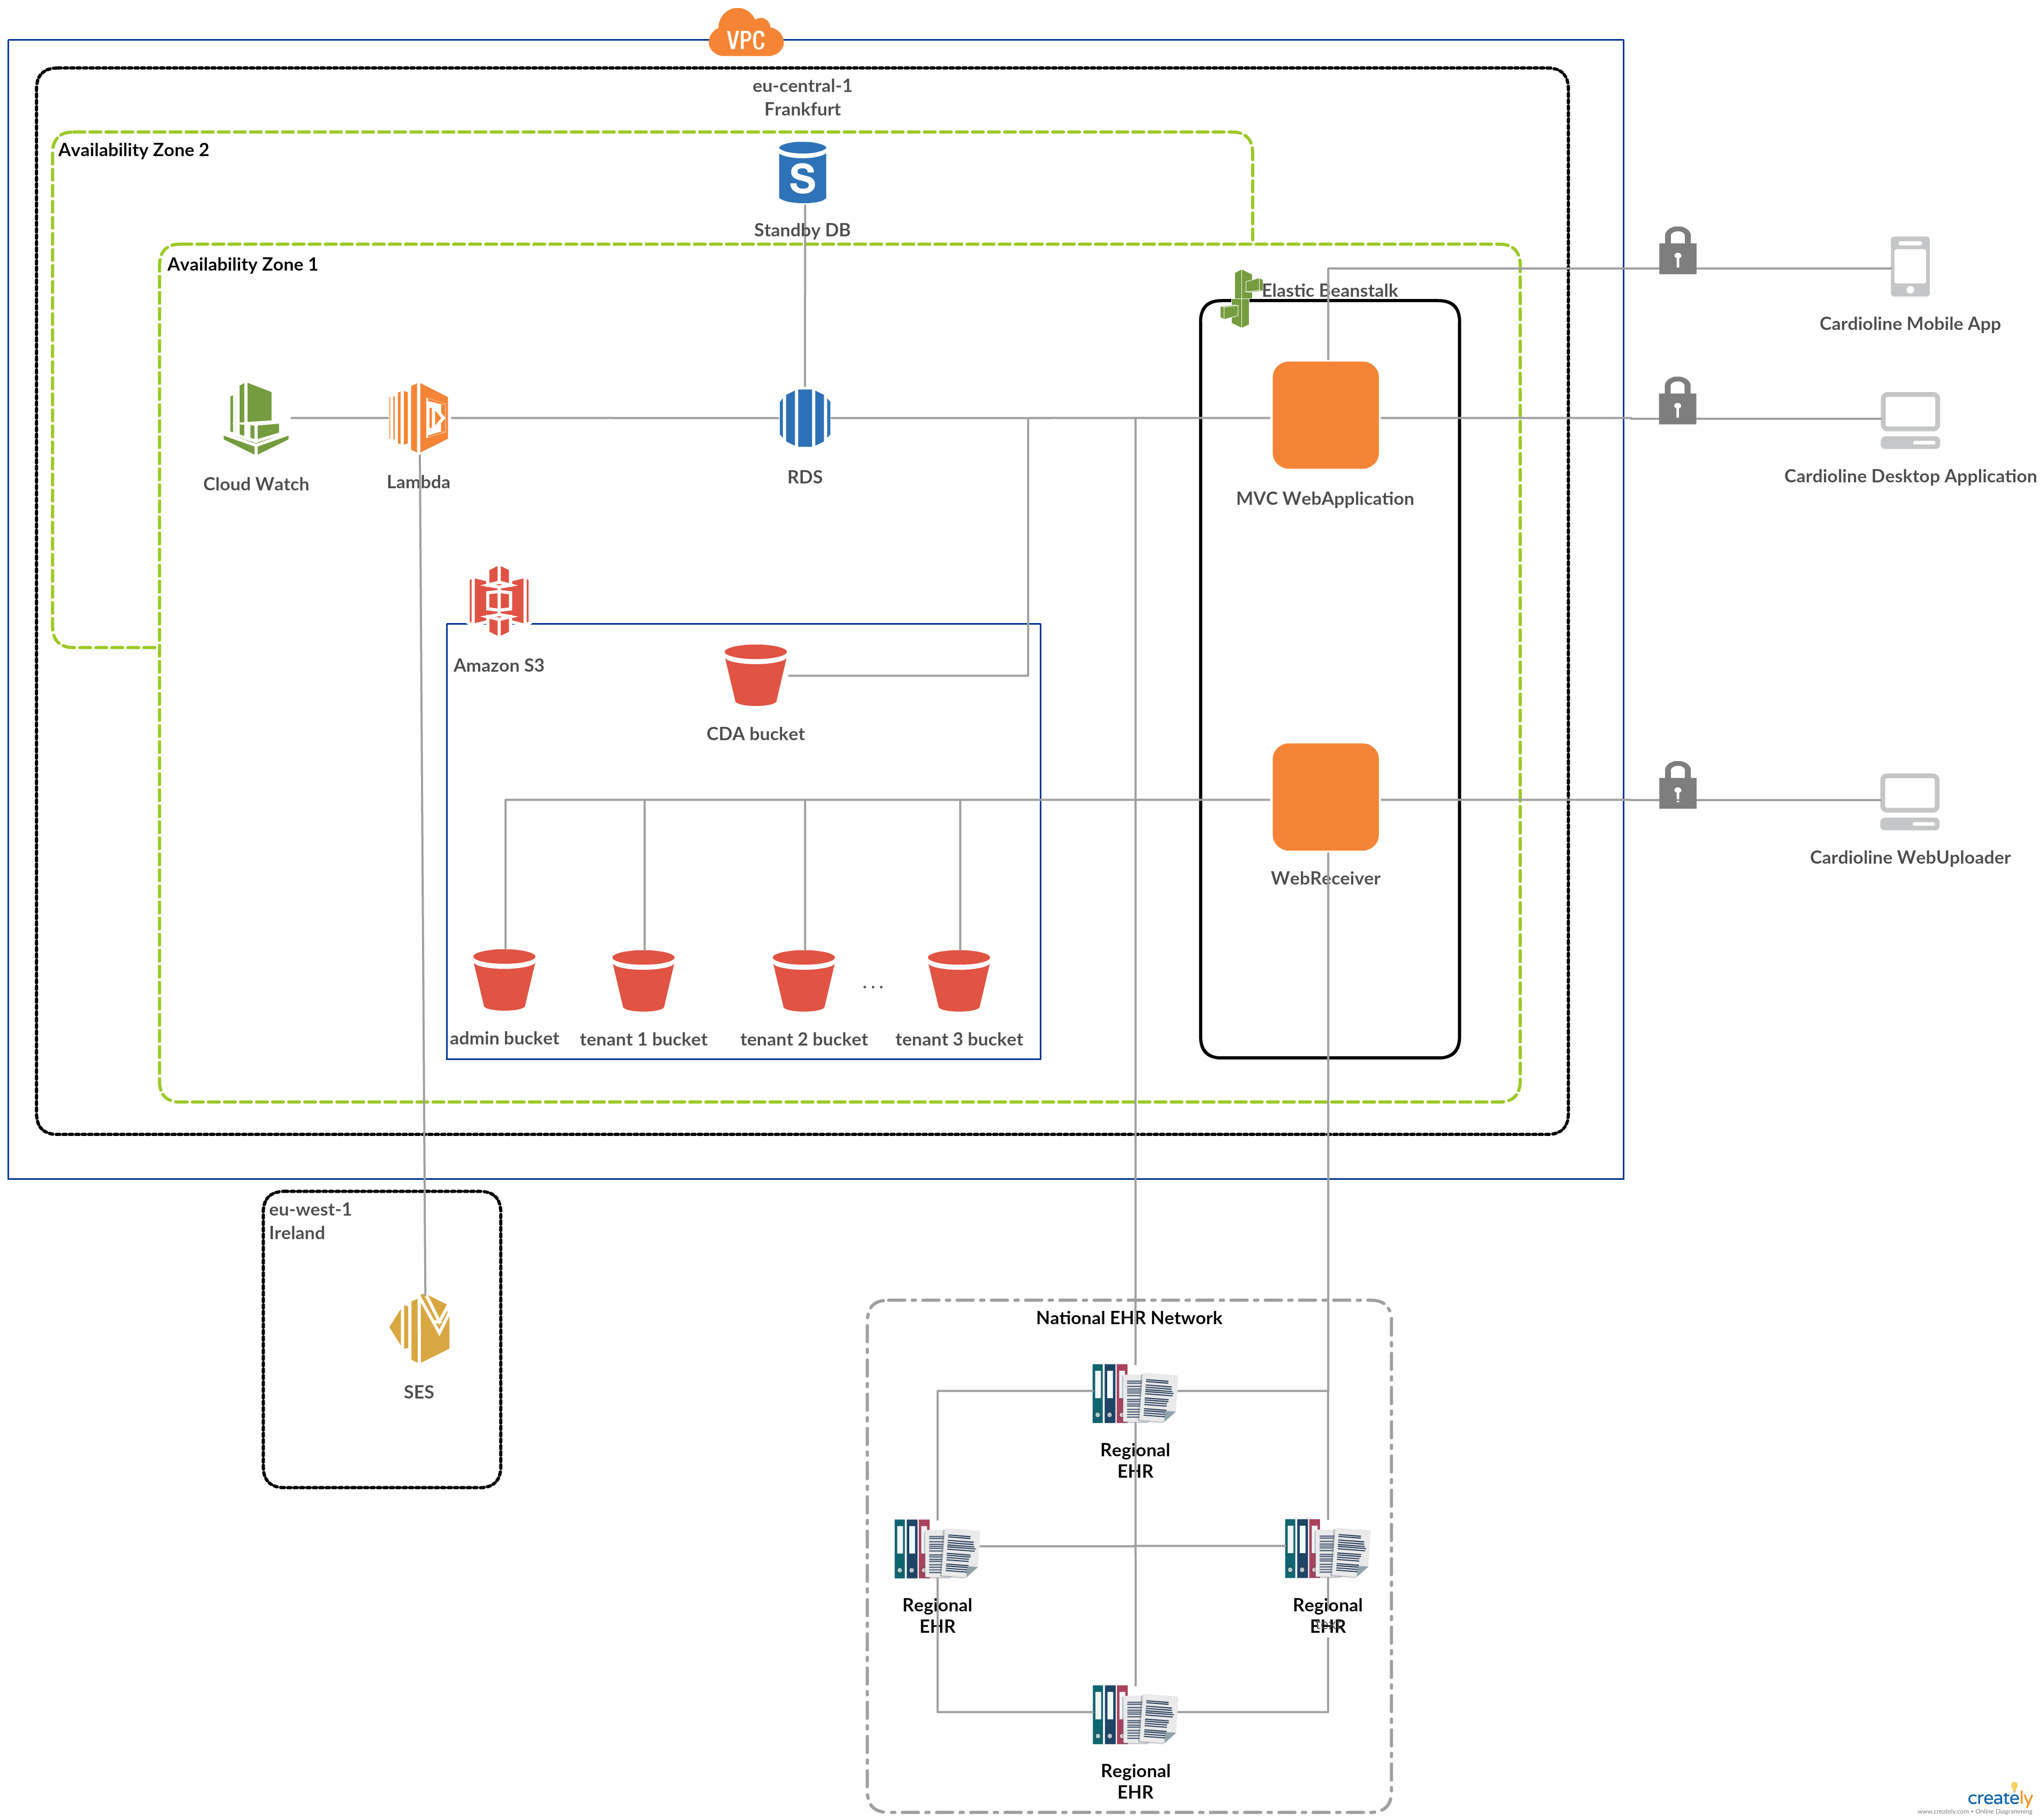
\includegraphics[width=\textwidth]{architecture}
    \caption{a nice plot}
    \label{fig:architecture}
\end{figure}
\section{Ecg Workflow}
\section{Notification}
\section{Interoperability of digital electrocardiograms data}
\subsection{Resting}
\subsection{Cardiac stress test}
\subsection{Holter}
\paragraph{Web Receiver}
\paragraph{Web Uploader}
\paragraph{S3 Bucket synchronization}